\section{Overview}

An automated regression test suite for \maestro\ (or any BoxLib-based
code) written in Python exists in {\tt BoxLib/Tools/C\_util/regtests/}
as {\tt testnew.py}.  The test suite consists of a set of problem
definitions (the \maestro\ problem + their inputs file, etc.).  When
the suite is run the first time, the plotfiles created at the end of
each problem's execution is stored as a benchmark.  After this
initialization, each subsequent run of the test suite compares the
current output of the code, level-by-level and zone-by-zone to the
stored benchmarks (using the {\tt fcompare.f90} routine in {\tt
  AmrPostprocessing/F\_Src/}).  Any differences are flagged as errors.
A web page report is generated by the test suite and provides a
history of the regression testing.  Single-processor and parallel test
problems, compilation tests, self-tests (problems that determine by
themselves whether they were successfully), and testing restarting
from a checkpoint file are supported.

\begin{figure}[t]
\centering
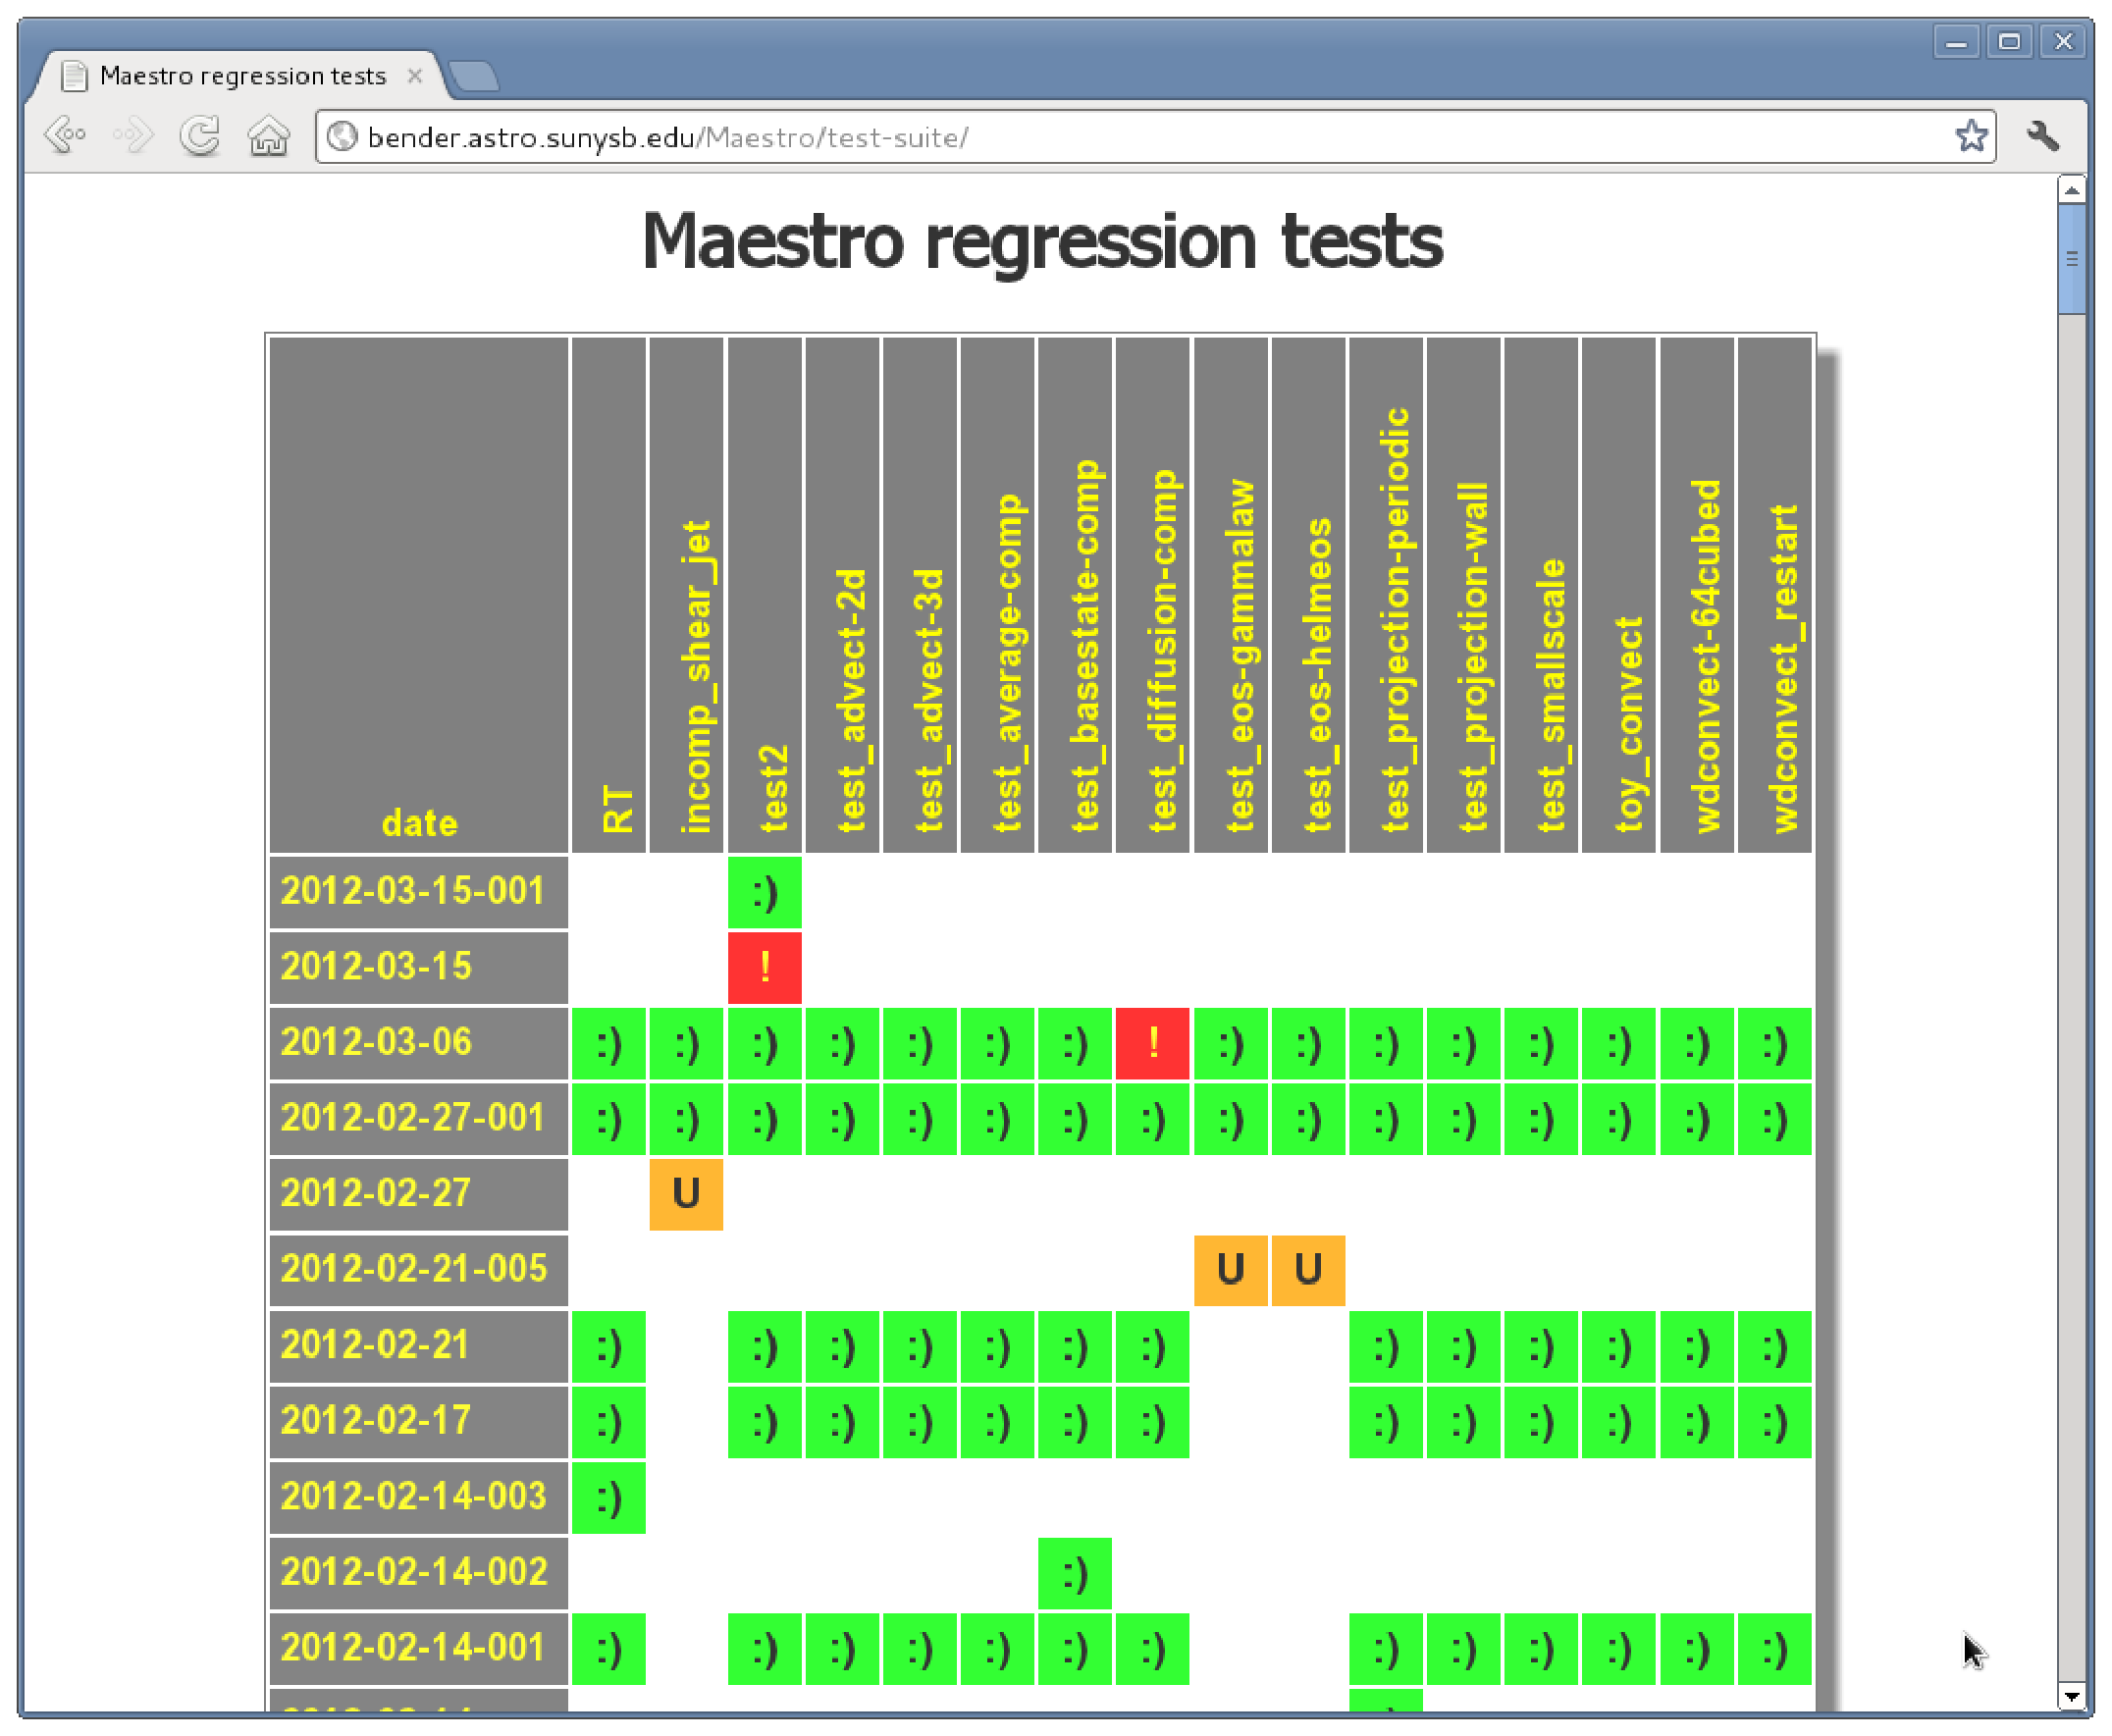
\includegraphics[width=5.0in]{\suitefigpath/testsuite}
\caption{\label{fig:test_suite_main} Main test suite results page.  Each 
row indicates a single test suite run, arranged by date, and each column
indicates a different test problem. }
\end{figure}

\section{Test Suite Inputs File}

The inputs file for the test suite separates the problems into blocks.
The header of a problem block has the form {\tt [problem-name]}.
Beneath each problem block, there are a number of options set for each
problem.  A separate heading, {\tt [main]}, is used for the suite-wide
options.

An example of the {\tt main} block from {\tt Maestro-tests.ini} is:
\begin{lstlisting}
[main]
boxLibDir      = /home/zingale/tests/BoxLib/
sourceDir      = /home/zingale/tests/MAESTRO/
testTopDir     = /home/zingale/tests/
webTopDir      = /home/www/Maestro/test-suite/
compareToolDir = /home/zingale/tests/AmrPostprocessing/F_Src/
helmeosDir     = /home/zingale/tests/MAESTRO/Microphysics/EOS/helmeos/

sourceTree = F_Src

suiteName = Maestro

FCOMP = gfortran

MPIcommand = mpiexec -n @nprocs@ @command@
\end{lstlisting}

The first group of options define the necessary paths.  Here, {\tt
  boxLibDir} points to the location of the \boxlib\ source, {\tt
  sourceDir} points to the top-level \maestro\ directory.  {\tt
  testTopDir} refers to the directory that the suite should use as its
root directory for running the tests and {\tt webTopDir} is the
directory in which to place the web output.  The {\tt fcompare.f90}
comparison tool source is expected to be found in {\tt
  compareToolDir}.  Finally, {\tt helmeosDir} lists the path to the
{\tt helm\_table.dat} file used by the general stellar equation of
state.

Next, we set {\tt sourceTree} to {\tt F\_Src}, indicating that
\maestro\ is built using the Fortran \boxlib\ framework.  This option
tells the test suite what build system to use.

{\tt FCOMP} tell the test suite which Fortran compilers to use.  These
override what is listed in any {\tt GNUmakefile} to ensure that the
compiler stays consistent in the tests.

The {\tt suiteName} option simply tells the test suite what name to
prefix to the output directories.  It does not need to match the
program name.  

Finally, {\tt MPIcommand} lists the generic manner in which to run an
MPI program on the target system.  If present, the string {\tt @host@}
in the {\tt MPIcommand} will be substituted by the {\tt MPIhost}
string by the test suite.  Similarly the {\tt @nprocs@} string will be
substituted by the number of processors, which is set on a
problem-by-problem basis.  Finally, the {\tt MPIcommand} should
include the string {\tt @command@}, which is where the
\maestro\ executable and inputs file will be substituted.  For single
processor runs, these options are ignored.

Each problem to be run by the test suite gets its own block.  For
example, a test listing for the {\tt test2} problem might look like:

\begin{lstlisting}
[test2]
buildDir = TEST_PROBLEMS/test2/
inputFile = inputs_2d
aux1File = model.hse.cool.coulomb
needsHelmEOS = 1
dim = 2
doVis = 1
visVar = ``tfromp''
compileTest = 0 
restartTest = 0
useMPI = 0
\end{lstlisting}

Here {\tt test2} contained inside the {\tt []} is the name of the
problem, as the test suite will refer to it.  {\tt buildDir} is the
path beneath {\tt sourceDir} where the {\tt make} command should be
executed.  The inputs file is given by {\tt inputFile} and the
necessary model file is listed by {\tt aux1File}. (Not all problems
will need this.  Additional auxiliary files can be specified via {\tt
  aux2File} and {\tt aux3File}).  Note that {\tt inputFile} and {\tt aux?File} are
specified relative to the {\tt buildDir}. The dimensionality is specified by {\tt dim}.

A number of options are available:
\begin{itemize}
\item  If the general stellar equation of state is
used, then {\tt needsHelmEOS} should be set to {\tt 1} to ensure that the
EOS table is linked into the run directory.  

\item {\tt link1File}, {\tt link2File}, and {\tt link3File} work like
the {\tt aux?File}s, but instead of copying the specified file into
the run directory, a symbolic link is made.

\item If the test is to be run in parallel,
the {\tt useMPI} should be {\tt 1} and {\tt numprocs} should give the number
of processors.  

\item To test the compilation of the problem only (and skip running),
set {\tt compileTest} to {\tt 1}.  

\item To test the ability of the code to restart, set {\tt restartTest} to
{\tt 1}.  Also set {\tt restartFileNum} to the number of the checkpoint file to restart
from.  The suite will run the problem as usual and then restart from the specified
checkpoint and run to completion again.  The output from the initial run will
then be compared to the output from the restart.  In a restart test, there
is no stored benchmark.

\item Some problems don't output plotfiles, but instead check internally
whether they are successful.  For these, set {\tt selfTest} to {\tt 1},
and set {\tt stSuccessString} to the string output to look for at the
end of the test to determine if it was successful.


\item To add a simple visualization to the test suite webpage, set
  {\tt doVis} to {\tt 1}, and set {\tt visVar} to the name of the
  plotfile variable to visualize.  An image of that field from the
  last plotfile will be appended to the problem's test webpage.


\item Ordinarily, the test suite uses the last plotfile output to compare to.
To force the comparison to a specific file, set {\tt compareFile} to the 
name of the file to compare to.

\item To override some of the options in the problem's {\tt GNUmakefile}
(e.g.\ use a different reaction network), set {\tt addToCompileString}
to the  string to add to the {\tt make} line that compiles the problem.

\end{itemize}



\section{Initializing the Test Suite}

The first time you run the test suite there are no benchmark files to compare to.
Once you generate an inputs file, as described above, you would simply run the
suite as: \\
$~~~~~${\tt ./testnew.py --make\_benchmarks "initial run" ./Castro\_tests.ini} \\
The string following {\tt --make\_benchmarks} is simply a comment that will
be added to the web report.
This command creates three output directories, using the {\tt suiteName} as the prefix.
\begin{itemize}
\item {\tt suiteName-tests} is where the tests are run.  Each time the test
 suite is run, a subdirectory, based on the date, is created, with a subdirectory
 for each test.  All the files necessary to run the test are copied into the
 test subdirectory.

\item {\tt suiteName-web} is where the web-based reports for the test are generated.
 The master webpage is {\tt suiteName-web/index.html}.

\item {\tt suiteName-benchmarks} is where the test benchmark files are stored.  This
 are used for comparison to the current output.
\end{itemize}



\section{Regular Use}

Once the initial benchmarks are created, you can compare the current
version of the code to the stored results by simply doing: \\
$~~~~~${\tt ./testnew.py ./Maestro\_tests.ini} \\ 
This will do a CVS/git update, generate {\tt ChangeLog} files listing all
of the CVS comments for the code, build the test comparison tools, and
then loop over each test, building and running the executable and
comparing the output to the benchmarks as required.

Upon completion of all the runs, a web page for this invocation of the
test suite will be generated as well as pages showing the details for
each of the problems run.  Test failures indicate that the current
output does not match the stored benchmarks.


\section{Updating Benchmarks}

A test failure means that the current version of the code gives a
different answer than the stored benchmark.  A test can fail either
because a bug was introduced into the code or a bug was fixed or new
feature introduced.

If a bug was introduced into the code recently, then by examining the
test history you can determine the time period in which the bug was
introduced.  The {\tt ChangeLog}s linked to on each test date's webpage
will list all the changes committed to CVS/git up to that point, which is
useful for tracking down the bug.  Once the bug is fixed, rerunning
the suite should generate a `pass'.

If a bug was fixed or a new feature was introduced, and you are
confident that the latest output is correct, then you can tell the
test suite to update the benchmarks.  If you want to do this for all
the test problems, you would do:\\
$~~~~~${\tt ./testnew.py --make\_benchmarks "X bug fixed" ./Castro\_tests.ini} \\
where the string after ``{\tt --make\_benchmarks}'' is a note that is listed
on the regression suite web page describing the reason for the benchmark
update.  Subsequent runs of the test suite will use the new benchmarks.
If you only want to update the benchmarks of a single test, then you
can use the ``{\tt --single\_test test}'' flag on the commandline, where
{\tt test} is the name of the test to update.

